En esta sección se detallarán los casos de uso y escenarios pertenecientes al subsistema de gestión de entradas del blog. La figura \ref{fig:casos_uso_subsistema_blog} muestra el diagrama de casos de uso del subsistema de gestión de debates.

\begin{figure}[h]
\centering
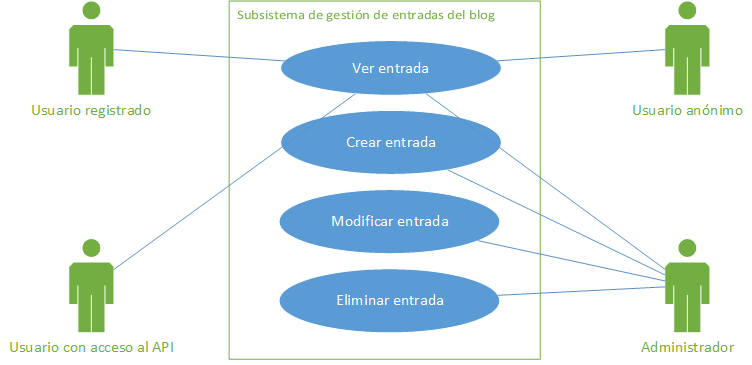
\includegraphics[width=\textwidth]{casos_uso_blog}
\caption{Diagrama de casos de uso del subsistema de gestión de entradas del blog}
\label{fig:casos_uso_subsistema_blog}
\end{figure}


\subsubsection{Caso de uso ``ver entrada''}
\begin{description}
\item[Descripción] 				El usuario quiere ver el contenido de una entrada del blog.
\item[Actores]					Cualquier rol de usuario.
\item[Escenario principal]	 	\hfill
								\begin{enumerate}
								\item El usuario accede al blog del Land Portal.
								\item Una vez en el blog, selecciona la entrada que quiere ver en detalle.
								\item El sistema carga la vista de la entrada mostrando tanto su contenido como sus comentarios.
								\end{enumerate}
\end{description}


\subsubsection{Caso de uso ``crear entrada''}
\begin{description}
\item[Descripción] El administrador quiere crear una nueva entrada en el blog del Land Portal.
\item[Actores] Administrador.
\item[Precondiciones] Haber iniciado sesión en el sistema.
\item[Escenario principal] \hfill
						 	\begin{enumerate}
							\item El administrador accede al blog del Land Portal.
							\item Una vez en el blog, el administrador pulsa el botón para crear una nueva entrada.
							\item Rellena los campos requeridos en el formulario de creación de la entrada.
							\item Rellena los campos opcionales que considere necesarios en el formulario de creación de la entrada.
							\item Pulsa el botón para guardar la entrada.
							\item El sistema guarda la entrada y la hace visible para todos los usuarios en el blog.
							\end{enumerate}
\item[Escenario alternativo 1] El administrador no ha rellenado todos los campos requeridos.
							\begin{enumerate}
							\item El sistema notificará al usuario de que faltan campos por rellenar.
							\item Se continuará desde el punto 3 del escenario principal.
							\end{enumerate}
\end{description}


\subsubsection{Caso de uso ``modificar entrada''}
\begin{description}
\item[Descripción] El administrador quiere modificar el contenido de una entrada del blog.
\item[Actores] El administrador del sistema.
\item[Precondiciones] Haber iniciado sesión en el sistema.
\item[Escenario principal] \hfill
						 	\begin{enumerate}
							\item El administrador accede al blog del Land Portal.
							\item Una vez en el blog, el administrador selecciona la entrada que quiere modificar.
							\item En la entrada correspondiente, el administrador pulsa el botón para editar su contenido.
							\item Rellena los campos requeridos en el formulario de modificación de la entrada.
							\item Rellena los campos opcionales que considere necesarios en el formulario de modificación de la entrada.
							\item Pulsa el botón para guardar los cambios
							\item El sistema actualiza los contenidos de la entrada del blog.
							\end{enumerate}
\item[Escenario alternativo 1]  No se rellenan todos los campos requeridos
							\begin{enumerate}
							\item El sistema informa al usuario del error y no modifica la información almacenada.
							\item Se continúa desde el punto 4 del escenario principal.
							\end{enumerate}
\end{description}

\subsubsection{Caso de uso ``eliminar entrada''}
\begin{description}
\item[Descripción] El administrador quiere eliminar una entrada del blog junto con todos sus comentarios.
\item[Actores] El administrador del sistema.
\item[Precondiciones] Haber iniciado sesión en el sistema.
\item[Escenario principal] \hfill
						 	\begin{enumerate}
							\item El administrador accede a la vista de administración.
							\item En la sección de contenidos localiza la entrada y pulsa el botón correspondiente para eliminarla.
							\item La entrada y sus comentarios serán eliminados del sistema.
							\end{enumerate}
\end{description}

